\documentclass[a4paper,11pt,openany]{book}
\usepackage[T1]{fontenc}
\usepackage[utf8]{inputenc}
\usepackage{lmodern}
\usepackage{hyperref}
\usepackage{graphicx}
\graphicspath{ {images/} }
\usepackage[english]{babel}

%%%%%%%%%%%%%%%%%%%%%%%%%%%%%%%%%%%%%%%%%%%%%%%%
% Chapter quote at the start of chapter        %
% Source: http://tex.stackexchange.com/a/53380 %
%%%%%%%%%%%%%%%%%%%%%%%%%%%%%%%%%%%%%%%%%%%%%%%%
\makeatletter
\renewcommand{\@chapapp}{}% Not necessary...
\newenvironment{chapquote}[2][2em]
  {\setlength{\@tempdima}{#1}%
   \def\chapquote@author{#2}%
   \parshape 1 \@tempdima \dimexpr\textwidth-2\@tempdima\relax%
   \itshape}
  {\par\normalfont\hfill--\ \chapquote@author\hspace*{\@tempdima}\par\bigskip}
\makeatother

%%%%%%%%%%%%%%%%%%%%%%%%%%%%%%%%%%%%%%%%%%%%%%%%%%%
% First page of book which contains 'stuff' like: %
%  - Book title, subtitle                         %
%  - Book author name                             %
%%%%%%%%%%%%%%%%%%%%%%%%%%%%%%%%%%%%%%%%%%%%%%%%%%%

% Book's title and subtitle
\title{\Huge \textbf{Simulating Starlings Murmuration}}\\ 
% Author
\author{\textsc{Deepanshu Jindal} \\ \textsc{Arpan Mangal}}


\begin{document}

\frontmatter
\maketitle

\tableofcontents
\listoffigures

\mainmatter

%%%%%%%%%%%
% Preface %
%%%%%%%%%%%
\chapter*{Preface}
This documents details the mathematical modelling and functional design for an application for simulating the flocking behaviour shown by Starlings: often known as Starlings murmuration.\\
\begin{figure}[h]
\centering
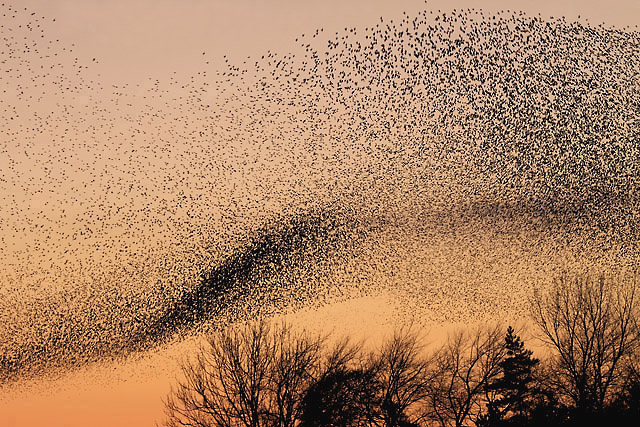
\includegraphics[scale=0.4]{Starling_murmuration.jpg}
\caption{Starlings murmuration}
\end{figure}
\\
Starlings murmuration is a type of swarm behaviour. From an abstract point of view, swarm behaviour is the collective motion of a large number of self-propelled entities. From the perspective of the mathematical modelling, it is an emergent behaviour arising from simple rules that are followed by individuals and does not involve any central coordination.\\

To model this we would use the boids program created by Craig Reynolds as an inspiration.
\\


\chapter{Mathematical Model}

\section{Intuition behind the model}
From the general observation of swarm behaviour we can identify some basic rules which we can assume that each member of the swarm is following:

1. Alignment : Move in the same direction as your neighbours

2. Cohesion : Remain close to your neighbours

3. Separation : Avoid collisions with your neighbours
\\
Apart from these basic rules, we can add in several assumptions such as they try to stay above a sleeping site, and when they happen to move outwards from the sleeping site, they return to it by turning. 


\section{Extension to the rules}
We bring in obstacle avoidance and wall avoidance properties so as to confine the boids to a certain section of the space.
\\
We add in random noise to the motion of each bird to bring in the effect of constant stirring motion.


\section{Quantification of the rules}
We mathematically describe the computation for a particular bird. Let there be \emph{n} birds in the flock.\\
Let the velocities and position vectors of birds be represented by $\vec{v_1},\vec{v_2},\vec{v_3} ... \vec{v_n}$ and $\vec{r_1},\vec{r_2},\vec{r_3} ... \vec{r_n}$ respectively. 
\end{document}
